\begin{figure}
	\centering
	\begin{tikzpicture}[scale=1.0]
	
		\node (A) at (-4,4) {
			\begin{tikzpicture}[scale=0.15]
				\draw[thick] (-6,2) -- (6,2);
				\draw[thick] (-6,-2) -- (6,-2);
				\draw[thick] (-2,-6) -- (-2,6);
				\draw[thick] (2,-6) -- (2,6);
				\draw[very thick] (-6,-6) -- (-6,6) -- (6,6) -- (6,-6) -- cycle;

				\node at (0,0) {\textcolor{blue}{$\bm{\times}$}};
				\node at (0,4) {\textcolor{blue}{$\bm{\times}$}};
				\node at (-4,4) {\textcolor{red}{$\bm{\bigcirc}$}};
				\node at (4,4) {\textcolor{red}{$\bm{\bigcirc}$}};
			
				\shade [ball color=green] (-4,0) circle [radius=0.75cm];
				\shade [ball color=yellow] (-4,-4) circle [radius=0.75cm];
				\shade [ball color=black] (0,-4) circle [radius=0.75cm];
				\shade [ball color=blue] (4,-4) circle [radius=0.75cm];
				\shade [ball color=orange] (4,0) circle [radius=0.75cm];
			\end{tikzpicture}
		};

		\node at (-2,4) {\footnotesize Move for \Large\textcolor{blue}{$\bm{\times}$}};

		\node (B) at (-4,0) {
			\includegraphics[scale=0.3]{14_rl/02_img/menace}
		};

		\node (C) at (2,0) {
			
\begin{tikzpicture}[scale=0.15]
				\shade [ball color=black] (0,0) circle [radius=2cm];
			\end{tikzpicture}
		};

		\node (D) at (2,4) {
			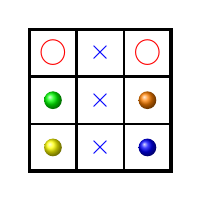
\begin{tikzpicture}[scale=0.15]
				\draw[thick] (-6,2) -- (6,2);
				\draw[thick] (-6,-2) -- (6,-2);
				\draw[thick] (-2,-6) -- (-2,6);
				\draw[thick] (2,-6) -- (2,6);
				\draw[very thick] (-6,-6) -- (-6,6) -- (6,6) -- (6,-6) -- cycle;

				\node at (0,-4) {\textcolor{blue}{$\bm{\times}$}};
				\node at (0,0) {\textcolor{blue}{$\bm{\times}$}};
				\node at (0,4) {\textcolor{blue}{$\bm{\times}$}};
				\node at (-4,4) {\textcolor{red}{$\bm{\bigcirc}$}};
				\node at (4,4) {\textcolor{red}{$\bm{\bigcirc}$}};

				\shade [ball color=green] (-4,0) circle [radius=0.75cm];
				\shade [ball color=yellow] (-4,-4) circle [radius=0.75cm];
				\shade [ball color=blue] (4,-4) circle [radius=0.75cm];
				\shade [ball color=orange] (4,0) circle [radius=0.75cm];
			\end{tikzpicture}
		};

		\draw[->,thick] (A) -- node[left,align=left] {\footnotesize Choose matchbox \\ \footnotesize according to position} (B);
		\draw[->,thick] (B) -- node[above,align=left] {\footnotesize Pick a marble \\ \footnotesize from the matchbox} (C);
		\draw[->,thick] (C) -- node[right,align=left] {\footnotesize Execute move \\ \footnotesize according to 
			\\ \footnotesize marble} (D);
	
	\end{tikzpicture}
\end{figure}